\documentclass[11pt]{article}

% ACL style in final (non-anonymous) mode. The style file discards table-of-contents lines, so the
% standard command is saved before it is loaded and restored after; page numbers are switched on for the page budget.
\let\vsaddcontentsline\addcontentsline
\usepackage[final]{acl}
\let\addcontentsline\vsaddcontentsline

\geometry{a4paper,left=2cm,right=2cm,top=2.1cm,bottom=2.1cm,heightrounded}
\setlength\columnsep{0.65cm}
\usepackage{times}
\usepackage{latexsym}
\usepackage[T1]{fontenc}
\usepackage[utf8]{inputenc}
\usepackage{microtype}
\usepackage{inconsolata}
\usepackage{graphicx}
\usepackage{booktabs}
\usepackage{array}
\usepackage{longtable}
\usepackage{float}
\usepackage{enumitem}
\newcolumntype{L}[1]{>{\raggedright\arraybackslash}p{#1}}
\usepackage{xcolor}
\usepackage{needspace}
\usepackage{multicol}
\usepackage{tikz}
\usetikzlibrary{positioning,fit,backgrounds,arrows.meta}
\hypersetup{hidelinks}
\renewcommand{\topfraction}{0.9}\renewcommand{\bottomfraction}{0.8}\renewcommand{\textfraction}{0.1}
\renewcommand{\floatpagefraction}{0.8}\renewcommand{\dbltopfraction}{0.9}\renewcommand{\dblfloatpagefraction}{0.8}
\setlength{\textfloatsep}{10pt plus 2pt minus 2pt}\setlength{\dbltextfloatsep}{10pt plus 2pt minus 2pt}
\pagestyle{plain}
\newcommand{\vs}{VS-Final}
% Run-in headings also go to the contents, without their closing period.
\def\vsstrip#1.\vsend{#1}
\newcommand{\para}[1]{\paragraph{#1}\addcontentsline{toc}{subsection}{\vsstrip#1\vsend}}
\setcounter{tocdepth}{2}
% Contents: sections bold, their sub-headings one per line below them, page numbers on the right.
\usepackage{titletoc}
\definecolor{vsblue}{HTML}{1F3A5F}
% Section headings in the same blue as the title page and the contents.
% (acl.sty's own definitions, with the colour added; spacing unchanged)
\makeatletter
\def\section{\@startsection {section}{1}{\z@}{-2.0ex plus
    -0.5ex minus -.2ex}{1.5ex plus 0.3ex minus .2ex}{\large\bfseries\raggedright\color{vsblue}}}
\def\subsection{\@startsection{subsection}{2}{\z@}{-1.8ex plus
    -0.5ex minus -.2ex}{0.8ex plus .2ex}{\normalsize\bfseries\raggedright\color{vsblue}}}
\makeatother
\renewcommand{\abstractname}{\color{vsblue}Abstract}
\titlecontents{section}[2.4em]{\addvspace{3pt}\bfseries}%
  {\contentslabel[{\color{vsblue}\thecontentslabel}]{2.4em}}{}%
  {\hfill\contentspage}
\titlecontents{subsection}[4.6em]{}%
  {\contentslabel{2.2em}}{}%
  {\hfill\contentspage}

\begin{document}

% ------------------------------------------------------------------ title page and contents (not counted)
\onecolumn
\pagenumbering{roman}
\thispagestyle{empty}
\begin{center}
\vspace*{3.8cm}
{\color{vsblue}\rule{\textwidth}{2.2pt}}\par
\vspace{0.9cm}
{\fontsize{26}{31}\selectfont\bfseries\color{vsblue} Vakeel-Sahayak.ai\par}
\vspace{0.35cm}
{\fontsize{17}{22}\selectfont A Multi-Agent Harness for\\[2pt] Evidence-Grounded Bail Drafting\par}
\vspace{0.9cm}
{\color{vsblue}\rule{\textwidth}{2.2pt}}\par
\vspace{0.5cm}
{\Large\scshape\color{vsblue} Technical Report\par}
\vspace{1.6cm}
{\large\bfseries Vishak Kashyap K\hspace{1.4em}Shravani K\hspace{1.4em}Satvik Rao\hspace{1.4em}Harshita Kumari\par}
\vspace{0.9cm}
{\large IIIT Hyderabad\par}
\vspace{0.2cm}
{\large CL3.410 Language Models and Agents\par}
\vspace{0.2cm}
{\large 15 November 2026\par}
\vspace{0.2cm}
{\large\color{vsblue}\url{https://github.com/vishakkashyapk30/lma-group-project}\par}
\vspace{2.6cm}
\resizebox{\textwidth}{!}{
\begin{tikzpicture}[font=\scriptsize, >=Stealth, line width=0.5pt, color=vsblue,
  ag/.style={draw, rounded corners=1.5pt, align=center, minimum width=1.6cm, minimum height=0.7cm, inner sep=2pt},
  gt/.style={draw, dashed, rounded corners=4pt, align=center, minimum width=1.2cm, minimum height=0.7cm, inner sep=2pt}]
\node[ag] (a1) at (0,0) {Pairokar};
\node[ag, right=0.3cm of a1] (a2) {Munshi};
\node[ag, right=0.3cm of a2] (a3) {Peshkar};
\node[gt, right=0.3cm of a3] (g1) {Gate 1};
\node[ag, right=0.3cm of g1] (a4) {Sutradhar};
\node[ag, right=0.3cm of a4] (a5) {Vakeel};
\node[ag, right=0.3cm of a5] (a6) {Abhiyojak};
\node[gt, right=0.3cm of a6] (g2) {Gate 2};
\foreach \x/\y in {a1/a2,a2/a3,a3/g1,g1/a4,a4/a5,a5/a6,a6/g2} \draw[->] (\x) -- (\y);
\end{tikzpicture}}
\end{center}
\vfill
\clearpage
\thispagestyle{plain}
{\color{vsblue}{\fontsize{20}{24}\selectfont\bfseries Contents}\par\vspace{4pt}\rule{\textwidth}{2.2pt}\par}
\vspace{2pt}
{\small\linespread{1.05}\selectfont\setlength{\parskip}{0pt}
\makeatletter\@starttoc{toc}\makeatother}
\clearpage

% ------------------------------------------------------------------ body (eight pages)
\twocolumn
\pagenumbering{arabic}

\begin{abstract}
Legal-aid lawyers in India prepare bail applications from short case files, and a brief helps only if it rests on the file and on real authorities. We ask whether a structured multi-agent harness (evidence contracts, per-sentence checks, a simulated prosecutor and two counsel approvals enforced in code) grounds bail drafting better than simpler retrieval on the same model, and which of its design decisions account for the gain. Vakeel-Sahayak.ai runs six agents over ten typed stores. Its first full system (Full) did not consistently beat seven simpler baselines on development orders; a failure analysis of retrieval, dossier completion, grounding and objection handling led to four modifications, and we selected the resulting system (\vs{}) on 50 development orders. We tested it once on 80 sealed public High Court orders (of 200 planned), with the facts part of each order as input and reference labels derived automatically from the rest of the order. Against Full, \vs{} raises objection recall from 0.52 to 0.73 and answerable coverage from 0.36 to 0.61 and lowers the share of argument sentences not entailed by the case facts (M6) from 0.99 to 0.89; it trades citation precision (0.85 to 0.71) and time per order (398 to 719 s) for these gains. Its fabricated-citation rate is 0.00, against 0.95 and 0.64 for the two baselines that retrieve comparably. Four of the five registered hypotheses hold. The gains accompany changes in how evidence, abstention and objections are handled, not a larger number of agents; validation with lawyers on real case files is the next step.
\end{abstract}

\section{Introduction}
\label{sec:intro}

A legal-aid lawyer preparing a regular bail application in an Indian High Court starts from a pile of documents: a High Court order, a scanned Sessions Court order, a phone photo of the first information report (FIR), remand orders and a custody certificate, often merged into one PDF and often in Hindi. This application needs five kinds of knowledge: exact statute text, the mapping from old to new sections after the 2024 change of criminal codes (IPC and CrPC to BNS and BNSS), court reasoning on each bail factor, the citation history of every authority, and the case timeline. No single search index serves all five.

Existing work covers parts of this task. Commercial legal research tools retrieve before they write, yet they still fabricate and misground citations \citep{magesh2025}, while work on Indian courts mostly predicts judgments or outcomes \citep{nigam2025nyayarag,nigam2024predex}. Adaptive retrieval lets a model critique what it retrieved or judge whether the context is sufficient \citep{asai2024selfrag,yan2024crag,jeong2024adaptive,joren2025sufficient}. Multi-agent methods add a critic or a debate, with mixed evidence: self-critique without an outside verifier helps little \citep{gou2024critic,huang2024selfcorrect}, voting partly explains debate gains \citep{choi2025debate}, and shared context can hurt \citep{wynn2025talk}.

These parts have rarely been tested together on legal drafting against simple baselines that use the same model. Our research question is whether a structured, specialised multi-agent architecture grounds bail drafting better than simpler LLM systems, and which architectural decisions account for any gain. The study followed the process below. We built a first full system (``Full'': planning, checking and adversarial review all switched on) and measured it against the baselines on development orders under three hosted model families, where it did not consistently outperform them. A failure analysis traced the weaknesses to retrieval planning, dossier completion, grounding checks and objection processing. We tested eight modifications on development orders, selected \vs{} (Full plus four of them), and evaluated it once on sealed orders, where it improves several measured outcomes over Full.

The report keeps four things apart. The \emph{intended application} is lawyer-supervised bail preparation from case documents. The \emph{evaluated task} is controlled bail drafting from the facts part of public High Court orders, scored against reference labels derived from other parts of the same orders; it tests the drafting harness, not the intake of messy client bundles. The \emph{demonstrated engineering} (document intake, a pseudonymisation boundary, two approval gates, typed stores, orchestration) is covered by tests and six synthetic demo cases, which show a working interface and workflow. Lawyer usefulness, filing quality and legal correctness on real client files are the \emph{next validation steps}; the system is a drafting aid for panel lawyers, junior advocates and supervised legal-aid clinics, and it does not predict outcomes, show grant rates, or advise accused persons or the public. Section~\ref{sec:limitations} collects the scope limits with their causes; the Glossary after the references defines every label.

In this paper, we describe the harness, the search that selected \vs{}, and one sealed test. Our contributions are:
\begin{enumerate}[label=(\arabic*),leftmargin=*,itemsep=1pt,topsep=3pt]
\item \textbf{A harness with approvals enforced in code.} Six agents work over ten typed stores, and counsel approves twice; on the sealed slice the code refused all 320 export attempts made before the second approval (Sections~\ref{sec:system} and~\ref{sec:results}).
\item \textbf{A failure-driven search with a holdout.} Four fixes derived from Full's failures give \vs{}, which on 30 development orders has 30 wins, 37 ties and 3 losses where Full has 11, 49 and 10, and repeats this on 20 held-out orders (22, 26, 3). Two candidates with more wins were rejected because they win by writing fewer or copied sentences (Section~\ref{sec:arch}).
\item \textbf{A sealed test with registered hypotheses.} On 80 orders opened once, four of five hypotheses hold and one is falsified on one cell; gains and trade-offs are reported together (Section~\ref{sec:results}).
\item \textbf{Robustness checks.} With reference labels from rules alone no verdict changes, and two fresh reruns on development orders keep the same three losses (Section~\ref{sec:results}).
\item \textbf{Ablations, with their scope.} Removing strict abstention costs \vs{} four comparisons and removing objection-by-id two; ablations that remove several switches at once are reported as combined effects (Section~\ref{sec:ablations}).
\item \textbf{Evaluation without manual annotation.} Reference labels come from court text through two independent labelers that must agree on a verbatim span (Section~\ref{sec:eval}).
\end{enumerate}

\section{System}
\label{sec:system}

We call the controlled scaffold around the language models the \emph{harness}: evidence contracts, per-sentence checks, approval gates and opt-in switches. Every part of this section describes one piece of it.

\para{A worked case.} We start with one development order, t1dev-019: an anticipatory bail petition in the Andhra Pradesh High Court with 871 characters of facts. The dossier agent finds ten fields unsupported in so short a record, and they become questions for counsel. The orchestrator plans five bail factors and queries the stores (115 store calls). The ground on a weak prima facie case cites \emph{Kunal v.\ State} (Delhi High Court, 2024, para 7), and the checker finds that the cited paragraph supports the sentence (entailment 0.99). The grounds on gravity and witness tampering each fail a first check on one sentence and are repaired against the retrieved authority. The ground on antecedents can only say that the record is silent, so it leaves the argument and becomes an open issue for counsel. The simulated prosecutor raises six objections (two answered, two partly answered, two unanswered). Scripted counsel approved the dossier but not the brief, and the system refused the export.

\begin{figure*}[t]
\centering
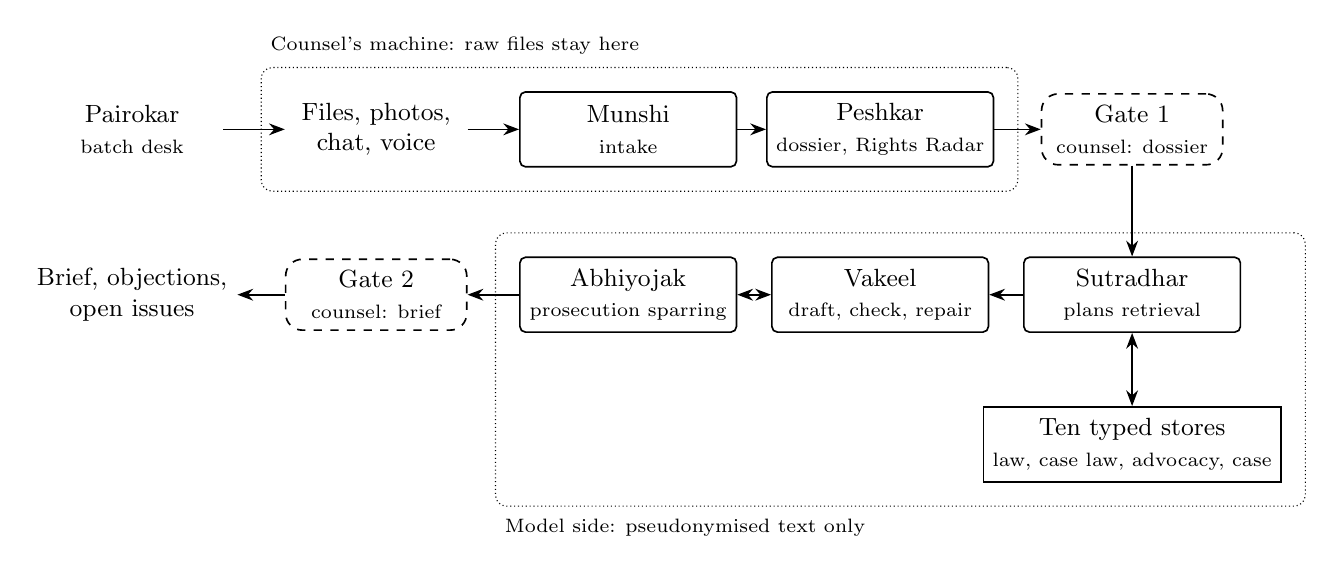
\begin{tikzpicture}[
  font=\small, >=Stealth, line width=0.6pt,
  ag/.style={draw, rounded corners=2pt, align=center, minimum width=2.75cm, minimum height=0.95cm},
  st/.style={draw, align=center, minimum width=2.75cm, minimum height=0.95cm},
  gt/.style={draw, dashed, rounded corners=6pt, align=center, minimum width=2.3cm, minimum height=0.9cm},
  io/.style={align=center, minimum width=2.3cm}]
\node[io] (pa) at (0,0) {Pairokar\\{\scriptsize batch desk}};
\node[io] (in) at (3.1,0) {Files, photos,\\chat, voice};
\node[ag] (mu) at (6.3,0) {Munshi\\{\scriptsize intake}};
\node[ag] (pe) at (9.5,0) {Peshkar\\{\scriptsize dossier, Rights Radar}};
\node[gt] (g1) at (12.7,0) {Gate 1\\{\scriptsize counsel: dossier}};
\node[ag] (su) at (12.7,-2.1) {Sutradhar\\{\scriptsize plans retrieval}};
\node[ag] (va) at (9.5,-2.1) {Vakeel\\{\scriptsize draft, check, repair}};
\node[ag] (ab) at (6.3,-2.1) {Abhiyojak\\{\scriptsize prosecution sparring}};
\node[gt] (g2) at (3.1,-2.1) {Gate 2\\{\scriptsize counsel: brief}};
\node[io] (out) at (0,-2.1) {Brief, objections,\\open issues};
\node[st] (stores) at (12.7,-4.0) {Ten typed stores\\{\scriptsize law, case law, advocacy, case}};
\draw[->] (pa) -- (in); \draw[->] (in) -- (mu); \draw[->] (mu) -- (pe); \draw[->] (pe) -- (g1);
\draw[->] (g1) -- (su); \draw[->] (su) -- (va); \draw[<->] (va) -- (ab); \draw[->] (ab) -- (g2); \draw[->] (g2) -- (out);
\draw[<->] (su) -- (stores);
\begin{scope}[on background layer]
 \node[draw, densely dotted, rounded corners, fit=(in)(mu)(pe), inner sep=0.3cm] (lap) {};
 \node[draw, densely dotted, rounded corners, fit=(su)(va)(ab)(stores), inner sep=0.3cm] (srv) {};
\end{scope}
\node[font=\scriptsize, anchor=south west] at ([yshift=1pt]lap.north west) {Counsel's machine: raw files stay here};
\node[font=\scriptsize, anchor=north west] at ([yshift=-1pt]srv.south west) {Model side: pseudonymised text only};
\end{tikzpicture}
\caption{The six agents, the two gates enforced in code (dashed) and the ten typed stores; dotted frames show where each part runs, and double-headed arrows are request and reply. The sealed evaluation of Section~\ref{sec:results} starts at Sutradhar with the facts text of each order and the dossier built from it; Munshi, Pairokar and the Rights Radar are covered by tests and the demo cases.}
\label{fig:arch}
\end{figure*}

\para{Six agents.} The case above passes through six agents, each named after a role in an Indian court office and each making one narrow decision (Figure~\ref{fig:arch}). \emph{Munshi} (intake) decides how to read and file each page. \emph{Peshkar} builds the dossier, a structured summary of the case with a source quote for every field, and the Rights Radar, which runs deterministic checks on custody periods and statutory rights. \emph{Sutradhar} (orchestrator) plans retrieval for each bail factor. \emph{Vakeel} (drafter) writes the grounds and checks and repairs every sentence. \emph{Abhiyojak} plays the prosecution, with its own prompt and its own stores. \emph{Pairokar} (batch desk) orders an office's files by urgency. The system appends every action to an event log, and the dossier, the brief and the sparring record are views of that log.

\para{Ten typed stores.} These agents search ten stores on four shelves, because each kind of knowledge needs its own search method. The \emph{law} shelf holds statutes (exact lookup) and the old-to-new section concordance (a typed graph). The \emph{case-law} shelf holds reasoning paragraphs, the citation graph and whole-order fact vectors. The \emph{advocacy} shelf holds defence arguments and prosecution objections by factor, which the system uses for coverage and never cites as authority. The private \emph{case} shelf holds the client's documents, a dated timeline and the dossier. The build has 161,708 reasoning paragraphs, 70,880 arguments, 55,161 objections and 5,842 citation edges.

\para{Evidence contracts.} For each of twelve bail factors, a contract tells Sutradhar what a ground needs: slots such as a co-accused order or an authority, whether each slot is required, the stores that may hold it, and a budget. The contract fixes what is needed and where it may be; Sutradhar decides the order of calls, the query, whether a result is sufficient and when to stop. A required slot that stays empty becomes an open issue for counsel, recorded in the event log with the slot name.

\para{Checks and gates.} Vakeel checks every sentence with a natural-language-inference model and with rules (statute lookup, section mapping, a good-law check), and repairs or flags the sentences that fail. Counsel then approves twice: Gate~1 for the dossier and Gate~2 for the brief. Only counsel can open a gate. Gate~2 is bound to a hash of the brief, so a later change closes it again, and no export is possible before it.

\para{Privacy boundary.} Raw client files stay on counsel's machine, and text reaches a hosted model only through a pseudonymisation boundary. The boundary replaces names and identifiers (FIR and case numbers, police stations, villages, addresses, vehicle numbers, ages) with aliases and shifts every date by a per-case offset. On the 250 orders of our main test set, no FIR number, case number or numeric date survived, and the boundary refused the 5 orders where OCR had glued names to other words. External model services are off by default, and the code locks paid providers.

\para{Evaluator demo and Hindi interface.} Six recorded synthetic cases (role pseudonyms, stamped pages, no real record) load when the API starts and let an evaluator walk the system without a key or a model call, through a guided, read-only tour of nine steps from the papers to the exported application; the Gate~2 step runs the real gate, so the export stays closed until the evaluator approves. The interface and the captions also run in Hindi. The cases demonstrate the interface and workflow; they are not an evaluation.

\section{Architectures We Tried}
\label{sec:arch}

\para{Search space.} Every design change is an opt-in switch in one typed configuration object, and the default leaves the output byte-identical. These switches fall into five families. \emph{Baselines} B0 to B6 are simpler systems on the same model: B0 to B3 make one model call with no retrieval or one retrieval step, B4 queries every store without a plan, B5 is a learned store router, and B6 is a rule template with no model (Table~\ref{tab:blind}). \emph{Ablations} A1 to A10 remove one part of Full. \emph{Variants} S1 to S18 each adapt one idea from a paper, such as self-critique retrieval (S1), sufficiency-based stopping (S3) or a three-role review (S11). \emph{Intake arms} P5 to P8 change how Munshi reads pages. \emph{Fixes} X1 to X8 came from our failure analysis below. The Glossary lists every label.

\para{What ran on which model.} We ran Full against the baselines on three hosted model families, and on none of them did it beat every baseline. On OpenAI \texttt{gpt-6-luna} (up to 38 development orders), Full's M6 was 0.87 to 0.89 against 0.82 to 0.87 for the baselines, and B4, which queries every store, had higher objection recall (0.90 against 0.75 on 20 orders). On the Gemini free tier (public court text only; 25 orders), Full led B0 to B3 on objection recall but not on M6. On Sarvam-105B (30 orders), Full's M6 was 1.00 against 0.90 to 0.96. No literature variant improved on Full on Sarvam, so the search started from Full on Sarvam-105B (Section~\ref{sec:limitations}).

\para{What the failure analysis found.} Reading Full's outputs on Sarvam revealed four causes. (1) M6 checks each argument sentence against the case facts alone, and 55\% of Full's flagged sentences state a legal principle from a cited authority; only about 9\% are real mismatches with the facts. (2) Intake and dossier filled about 2.8 of 13 dossier fields per case, so the planner never proposed grounds on custody period, parity or trial delay. (3) The system kept Abhiyojak's objections only if they named offered material by an exact store label: Full kept 66 objections and discarded 230, and 263 of 320 dropped references named a paragraph that had in fact been offered. (4) Sentences that failed the check stayed in the argument, marked, instead of becoming open issues.

\para{Protocol.} We tested eight fixes for these causes under a protocol that separates selection and test. The 30 development orders t1dev-000 to 029 are the \emph{search} orders, where we compared single switches and then combinations. The 20 orders t1dev-030 to 049 are a \emph{holdout}, which we ran once for the chosen system, Full and the baselines. We kept the 80 \emph{blind} orders of the test set sealed until we froze the code and hypotheses under the tags \texttt{prereg-v1} and \texttt{eval-freeze-v1} on 9 November. Our decision rule follows Section~\ref{sec:eval}: fewest losses against B0 to B6 on the quality metrics, then most wins.


\para{Outcome.} \vs{}, which combines Full with X1, X4, X5 and X7, achieves 30 wins, 37 ties and 3 losses on the search orders where Full has 11, 49 and 10 (Table~\ref{tab:cands} in the appendix). Objection recall (the share of the real prosecution's objections that the simulated prosecutor also raises) rises from 0.36 to 1.00. Coverage (the share of grounds emitted without a decline) rises from 0.64 to 0.97, and answerable coverage (the share of answerable factors with a supported argument) rises from 0.38 to 0.61. M6 falls from 0.99 to 0.90. On the holdout, the result repeats with the same three losses: 22, 26 and 3 for \vs{} against 10, 40 and 5 for Full (Table~\ref{tab:wlt_full} in the appendix).

\para{Candidates we rejected.} Three candidates have more wins than \vs{} and were rejected after we read their outputs. \emph{\vs{} minus X1} has 38 wins, but head to head it differs from \vs{} on two cells only (1 win, 18 ties, 1 loss): it wins the count of unsupported sentences because it writes fewer sentences (5.1 against 6.8 per order, with the same number supported). \emph{\vs{} with the free planner}, where the model plans without evidence contracts, has 38 wins and 1 loss. Three read-only checks of its saved outputs found that the gains come from measurement: it records no plan, so the unfinished-factor metric has nothing to count (88 contract gaps passed to counsel become 1), and its model rarely searches the precedent stores, so the drafter restates the facts under the factor headings (18\% of its grounds cite an authority against 90\%; 19 of 30 briefs cite none). \emph{\vs{} plus X8}, which replaces a paraphrased fact with the record sentence, adds one loss for three wins. Two single fixes did not help: X2 (case facts as near-verbatim spans) left most grounds empty on Sarvam (coverage 0.199), and X3 (one more prosecutor call) added objections without raising recall.

\para{Losses of \vs{}.} The three losses of \vs{} on the search orders are structural, and we did not chase them. \vs{} loses the unfinished-factor share (planned factors that stop with a required slot unfilled) to B4 and B5 because those baselines have no required slots and score near zero by construction. A search of the facts text finds none of the 62 missing slots (47 of 130 planned factors) stated in the record, so ``missing'' is the true state. It loses the doubly unsupported rate (defined in Section~\ref{sec:eval}) to B4 because B4 emits only 7.5\% of its grounds, a selected few sentences. Over all 50 development orders it also loses coverage to B6, a template that scores 1.00 by construction, and the doubly unsupported rate to B5.

\section{Final Method}
\label{sec:method}

\vs{} adds four switches to Full, and each switch answers one cause of Section~\ref{sec:arch}.

\para{X1, dossier gaps from the facts.} When the dossier lacks a field, the factor picker reads the raw facts text with rules (such as wider patterns for custody periods) and offers the facts text to the drafter for that factor. X1 answers cause (2): a dossier with 2.8 of 13 fields starved the planner.

\para{X4, strict abstention.} A sentence that still fails after repair, or a sentence that only says the record is silent, leaves the argument and becomes an open issue for counsel; the system does not emit an empty ground. X4 answers cause (4). Alone, it was the strongest single switch: coverage rose from 0.643 to 1.000 and answerable coverage rose from 0.379 to 0.530.

\para{X5, draft from the facts.} Vakeel drafts from the raw facts text, while the dossier still drives the planner and Gate~1. X5 was the only single switch that lowered M6 with an interval excluding zero ($-0.100$, 95\% interval $-0.150$ to $-0.053$ against Full); it ties sentences less tightly to each cited paragraph, so citation precision moves from 0.82 to 0.68 on the search orders for \vs{}, and \vs{} uses 27\% more tokens than Full.

\para{X7, objections resolved by id.} When an objection names offered material under the wrong store label, the system resolves it by the material's id instead of discarding it. X7 answers cause (3) and lifted objection recall from 0.364 to 1.000 on the 11 search orders with reference objections: the objections had been there and were being thrown away.

\para{Sparring reserve (after the freeze).} In the product, an opt-in switch (\texttt{sparring\_reserve\_tokens}, 200000) gives Abhiyojak and the reply step their own token pool, and the system judges each reply right after drafting it; an objection the pool cannot cover goes to counsel marked \texttt{NOT\_REPLIED\_BUDGET}. The reserve is outside the frozen system. On the 30 development search orders (one run per arm, Sarvam-105B) the judge graded 227 of 233 objections (97\%) with the reserve against 53 of 207 (26\%) without it, and 130 of 233 (56\%) received a reply judged answered or partly answered, against 23 of 207 (11\%). The reserve costs 26\% more tokens per order (120{,}643 to 151{,}434) and ran out in no order. Of 20 quality metrics compared in pairs, only over-search differs significantly (higher with the reserve, 0.0107 to 0.0258); objection recall rises from 0.73 to 1.00 without reaching significance (interval $[0.00, +0.55]$, $p=0.061$). This is exploratory evidence of a mechanism (Section~\ref{sec:limitations}).

\section{Evaluation Setup}
\label{sec:eval}

\para{Data.} All data come from public court text, official tables, existing datasets or constructed cases; we use no client data. Our corpus is Open India Law: of 115,988 bail-related orders read, 115,524 feed the stores. The main test set, T1, has 200 High Court orders from the test window (2024 onwards) and 50 development orders. The system reads the facts part of an order, and we derive reference labels from the rest of the same order. No public bail corpus annotated by legal experts exists, which is why labels come from the orders themselves. Eight further sets (T2 to T9) cover intake, rights rules, batching and more; this report uses T1.

\para{Automatically derived reference labels.} We make no labels by hand, and no model acts as a judge to score outputs (the code and artefacts call these labels ``gold''). For the factors the defence argued and for dossier fields, two labelers work independently: keyword and date rules, and a hosted model (\texttt{gpt-6-luna}) that does not see the rule output. A label enters the \emph{agreed labels} only if both agree and the model quotes a verbatim span found in the order. Agreement on the 250 orders is $\kappa=0.60$ for factors (95\% interval 0.55 to 0.64) and 0.84 for fields; a second model labeler (Sarvam-105B) on 80 random orders gives $\kappa=0.78$ on factors against the first. We also score against \emph{rule-only labels} as a declared second source. Three properties of this construction set the scope of the metrics. Agreement filtering favours clear-cut cases: 81 of 250 orders have no agreed factor and 88 have an agreed objection, so the recall metrics rest on those orders. A judicial order records what the court discussed, which need not be every appropriate defence argument. And the two model labelers agree with each other ($\kappa=0.78$) more than either does with the rules (0.59), so agreement shows consistency, not correctness. The metrics are therefore proxies for drafting quality; validation of the labels by legal experts is future work.

\para{Leakage control.} Orders before 2024 feed the stores. We exclude test orders and orders that share an FIR with them (464 in all) from every store, and an 8-word-overlap check compares each test order's facts with every store paragraph. The 80 blind orders were drawn with a seed and hashed before the freeze; the other 120 test orders were not run (D1).

\para{Baselines.} Seven baselines use the same model, the same 12-factor checklist and the same pseudonymised facts as our system (Table~\ref{tab:blind}). B0 to B3 make one model call; B4 and B5 use the tools and stores without contracts and serve as the baselines of comparable capability; B6 is a rule template with no model.

\begin{table}[t]
\centering\small
\setlength\tabcolsep{3.5pt}
\begin{tabular}{@{}lL{3.55cm}cc@{}}
\toprule
 & Baseline & \vs{} & Full \\
\midrule
B0 & single pass, no retrieval & 4/8/0 & 3/7/2 \\
B1 & one store, top 10, one call & 6/10/0 & 4/12/0 \\
B2 & whole-order retrieval & 7/12/0 & 4/14/1 \\
B3 & naive chunk retrieval & 7/9/0 & 5/10/1 \\
B4 & every store, fused, no plan & 10/9/2 & 6/11/4 \\
B5 & learned store router & 7/15/2 & 4/15/5 \\
B6 & expert rule template & 5/6/1 & 3/7/2 \\
\midrule
 & Total & \textbf{46/69/5} & 29/76/15 \\
\bottomrule
\end{tabular}
\caption{Wins/ties/losses of each system against each baseline on the 80 sealed orders. Each cell counts metric-by-baseline comparisons among the 25 quality metrics (paired bootstrap, Holm at 0.05 within each system, baseline set and metric); the totals count comparison outcomes, not orders or independent trials. Per system, 13 further cells have too few pairs and 42 are undefined.}
\label{tab:blind}
\end{table}

\para{Metrics.} We score 25 quality metrics, defined in Table~\ref{tab:metrics} of the appendix: among them factor recall, objection recall, coverage, answerable coverage, citation precision and recall in the style of ALCE \citep{gao2023alce}, and fabricated citations. Four metrics need a precise reading. \emph{M6}, the unsupported-fact rate, is the share of argument sentences that MiniCheck \citep{tang2024minicheck} does not find entailed by the facts of the case (the scorer refuses to use the system's own checker). Argument sentences also state legal propositions that rest on cited authorities, and case facts cannot entail those by nature, so M6 is not a hallucination rate: it measures how much of a brief the facts alone support. \emph{M6a} applies the same rule to case-fact sentences only; it is narrower and still relies on an automated entailment checker, so we report it beside M6. The \emph{fabricated-citation rate} is the share of citations whose id is absent from the index or whose quoted span is not found verbatim, so it tests validity; \emph{citation precision} tests whether the cited paragraph supports the sentence. A rate of 0.00 on the first says nothing about the second, and ``unsupported'' (not entailed), ``unverifiable'' and ``legally incorrect'' are different properties; the scorers establish only the first. The \emph{doubly unsupported rate} is the share of emitted sentences that MiniCheck finds supported neither by the facts nor by the rest of the same order (the code calls it \texttt{confident\_wrong\_rate}); it does not establish that a sentence is legally wrong, since an order need not restate every proposition it relies on. We judge cost (tokens, store calls, seconds) only against B4 and B5.

\para{Statistics.} Our unit of analysis is the order. We compare a system with a baseline on each metric using a paired bootstrap of the mean difference with 10,000 resamples. For each system and metric, the seven baselines form one family under Holm's correction at 0.05, so the correction operates within these families and the total win count is not a single hypothesis test. A comparison is a \emph{win} or a \emph{loss} only when the interval at its Holm level excludes zero; otherwise it is a \emph{tie}. We mark a cell with fewer than five paired orders as ``too few'', and a metric the baseline cannot produce (such as objection precision when it raises no objection) as ``undefined'', not won. Metrics defined on a subset of orders carry their own sample size: on the sealed slice factor recall rests on 9 orders, objection recall on 25, answerable coverage on 32 and M6a on 43 for \vs{}.

\para{Pre-registration.} We fixed the claims, metrics, seeds and decision rule in a pre-registration before opening the blind slice. We added five hypotheses for \vs{} (H-A1 to H-A5, Table~\ref{tab:hyp}) to the pre-registration before the opening. Table~\ref{tab:hyper} lists the settings and budgets. Fourteen numbered deviations (D1 to D14) record every departure from the registered plan, with date and reason (Table~\ref{tab:dev}).

\section{Results}
\label{sec:results}

\para{Main result.} On the 80 sealed orders, \vs{} improves on Full in the registered dimensions (Table~\ref{tab:means}). Objection recall rises from 0.52 to 0.73 ($+0.215$, paired 95\% interval $+0.024$ to $+0.400$, 25 orders), answerable coverage from 0.36 to 0.61 ($+0.250$, $+0.109$ to $+0.406$, 32 orders), and M6 falls from 0.99 to 0.89 ($-0.098$, $-0.135$ to $-0.063$, 79 orders). The doubly unsupported rate falls from 0.97 to 0.87 ($-0.101$, $-0.143$ to $-0.062$). Citation precision falls from 0.85 to 0.71 ($-0.133$, $-0.209$ to $-0.060$, 77 orders) and citation recall by a similar amount, because drafting from the facts ties sentences less tightly to the cited paragraphs; the unfinished-factor share rises from 0.17 to 0.40 because the system lists unmet factors for counsel instead of filling them. M6a is 0.43 for \vs{} (43 orders) and 0.75 for Full (27 orders); on the 16 orders where both are defined, the paired difference is $-0.161$ with an interval from $-0.443$ to $+0.115$, so the paired comparison does not separate them. Against the seven baselines, \vs{} has 46 wins, 69 ties and 5 losses over 120 metric-by-baseline comparisons (Table~\ref{tab:blind}); Full has 29, 76 and 15. These counts summarise comparison outcomes and are not a measure of application quality. \vs{} loses nothing to the one-call baselines B0 to B3; its five losses go to B4 and B5 (two each) and to the template B6 (one). Head to head, \vs{} has 8 wins, 13 ties and 3 losses against Full; the three losses are citation precision, citation recall and the unfinished-factor share.

\begin{table}[t]
\centering\small
\setlength\tabcolsep{3pt}
\begin{tabular}{@{}lL{3.0cm}L{3.15cm}@{}}
\toprule
 & Hypothesis for \vs{} & Sealed slice \\
\midrule
H-A1 & no loss to B0--B6 outside four cells declared structural & \textbf{falsified}: one further loss, unsupported-sentence count vs B5 (6.0 vs 4.2) \\
H-A2 & beats Full on objection recall and answerable coverage & \textbf{holds}: 0.52 to 0.73; 0.36 to 0.61 \\
H-A3 & beats B4 and B5 on citation precision and fabricated citations & \textbf{holds}: 0.71 vs 0.02 and 0.10; 0.00 vs 0.95 and 0.64 \\
H-A4 & unsupported-fact rate (M6) not worse than any baseline's & \textbf{holds}: 0.89 vs 0.94 to 1.00, a win over all seven \\
H-A5 & fewer store calls than B4 & \textbf{holds}: 110 vs 188 \\
\bottomrule
\end{tabular}
\caption{Four of the five registered hypotheses hold on the sealed slice. The four structural cells of H-A1 are the unfinished-factor share against B4 and B5, the doubly unsupported rate against B4 and coverage against B6; all four are losses, as declared.}
\label{tab:hyp}
\end{table}

\begin{table*}[t]
\centering\small
\setlength\tabcolsep{4.5pt}
\begin{tabular}{@{}lrrrrrrrrrrrr@{}}
\toprule
 & Obj. & Answ. & Cover- & M6 & M6a & Sent- & Unsup. & Cit. & Fabr. & Unfin. & Doubly & Store \\
System & recall & cov. & age & & & ences & count & prec. & cit. & factors & unsup. & calls \\
 & $\uparrow$ & $\uparrow$ & $\uparrow$ & $\downarrow$ & $\downarrow$ & & $\downarrow$ & $\uparrow$ & $\downarrow$ & $\downarrow$ & $\downarrow$ & $\downarrow$ \\
\midrule
\textbf{\vs{}} & 0.73 & 0.61 & 0.92 & 0.89 & 0.43 & 7.0 & 6.0 & 0.71 & 0.00 & 0.40 & 0.87 & 110 \\
Full & 0.52 & 0.36 & 0.70 & 0.99 & 0.75 & 7.3 & 7.1 & 0.85 & 0.00 & 0.17 & 0.97 & 103 \\
\midrule
B0 & 0.00 & 0.06 & 0.47 & 0.95 & -- & 8.2 & 7.7 & 0.00$^\dagger$ & 1.00$^\dagger$ & -- & 0.93 & 0 \\
B1 & 0.00 & 0.03 & 0.29 & 0.97 & -- & 5.9 & 5.7 & 0.00 & 0.00 & -- & 0.95 & 1 \\
B2 & 0.00 & 0.09 & 0.49 & 0.97 & -- & 9.8 & 9.4 & 0.00 & 0.80 & -- & 0.92 & 1 \\
B3 & 0.00 & 0.03 & 0.24 & 0.96 & -- & 4.2 & 4.0 & 0.00 & 0.00 & -- & 0.94 & 1 \\
B4 & 0.36 & 0.20 & 0.07 & 0.94 & 0.87 & 16.1 & 15.0 & 0.02 & 0.95 & 0.01 & 0.47 & 188 \\
B5 & 0.35 & 0.23 & 0.09 & 0.94 & 0.64 & 4.4 & 4.2 & 0.10 & 0.64 & 0.00 & 0.62 & 89 \\
B6 & 0.00 & 0.00 & 1.00 & 1.00 & -- & 7.8 & 7.7 & -- & -- & -- & 0.93 & 2 \\
\bottomrule
\end{tabular}
\caption{Key task metrics on the 80 sealed orders: \vs{} has the best objection recall, answerable coverage and M6 of all systems, and the highest citation precision among the systems other than Full. Means per order, each over the orders where the metric is defined (objection recall 25, answerable coverage 32, M6a 43 for \vs{} and 27 for Full; citation columns 5 to 12 orders for B1 to B3). ``Doubly unsup.'' is the doubly unsupported rate (Section~\ref{sec:eval}). ``--'': the system cannot produce the metric; $\dagger$: one order. Arrows give the better direction.}
\label{tab:means}
\end{table*}

\para{Hypotheses.} Four of the five registered hypotheses hold (Table~\ref{tab:hyp}). \vs{} beats B4 and B5 on citation precision (differences $+0.691$ and $+0.724$) and on fabricated citations: B4 and B5 fabricate at rates of 0.95 and 0.64, whereas \vs{} fabricates at 0.00. Its M6 beats all seven baselines (differences of $-0.05$ to $-0.12$; the interval against B0 is $-0.100$ to $-0.001$), and it needs 41\% fewer store calls than B4. H-A1 is falsified on one cell beyond the four declared structural: \vs{} loses the count of unsupported sentences to B5 ($+1.875$ per order, interval $+0.875$ to $+3.067$). Length explains this loss, since B5 writes 4.4 sentences per order against 7.0, and on the rate \vs{} beats B5. These verdicts stay the same when we keep errored records as scored and when we drop the two cases rerun under deviation D7.

\para{Cost and latency.} \vs{} gains these quality measures at a price in time (Table~\ref{tab:cost} in the appendix). Per sealed order it takes 719 s, against 398 s for Full, 269 s for B4 and 160 s for B5; it uses 122,387 tokens against 98,814, 120,614 and 79,877, and 110 store calls against 103, 188 and 89. Retrieval-call efficiency and system efficiency differ: \vs{} issues 41\% fewer store calls than B4 and a tied token count, but runs 2.7 times as long, because contracts, per-sentence checks, repairs and the sparring step add sequential model calls. Seconds are wall-clock on a hosted endpoint with several runs in parallel (D7), so they fix an order of magnitude. About twelve minutes per order suits overnight batch preparation; use in a legal-aid office has not been studied.

\para{Label source (D11) and reruns (D12).} The conclusions do not hinge on the model labeler. We scored the same saved outputs once more against the rule-only labels with the same scoring code: \vs{} has 45 wins, 70 ties and 5 losses (agreed labels: 46, 69, 5) and Full has 29, 74 and 17; five of 350 cells change outcome, and all five hypothesis verdicts remain unchanged. In an exploratory check of run-to-run spread, two reruns of all nine systems on the 30 search orders (frozen code, cache off) give \vs{} 30/31/3 and 35/28/3 (original 30/37/3) with the same three losses each time, while Full's losses move between runs (10/47/7 and 11/47/8).

\para{Tools and approvals.} \vs{} calls its tools with few bad arguments, and no export ran without approval (Table~\ref{tab:tools} in the appendix). \vs{} makes about 149 tool calls per order over 17 tools, and the system refuses 1.0\% for a bad argument, against 3.1\% for Full and 4.9\% and 6.4\% for B4 and B5. A refused call returns a typed error, and every order still ends with a complete brief. Each of the four tool-using systems tries one export per order before Gate~2: the code refuses all 320 attempts, giving an unapproved-action rate of 0 of 320. The privacy boundary refused 175 of \vs{}'s outgoing payloads that still carried a personal name. The errors row of Table~\ref{tab:tools} counts every typed error in the log, mostly expected refusals (Appendix~\ref{app:cost}).

\section{Ablations}
\label{sec:ablations}

\para{What the ablations isolate.} The twelve ablations of Table~\ref{tab:abl_full} (appendix) fall into three groups. The first removes one switch from \vs{}: minus X1, X4, X5 and X7, plus the single substitutions A3, A4, A6 and A7. Among them, removing strict abstention (X4) costs four wins and gains none, and removing objection-by-id (X7) costs two; removing X5 changes no cell, although X5 alone lowered M6 in the single-switch round, so X4 and X1 now cover most of that effect; removing X1 gives one win and one loss, which is the count effect from Section~\ref{sec:arch}. The second group, A1, A2, A8 and A9, cannot be run on top of all four switches, because the switch validator refuses the combinations; each of them removes a part together with the switch that depends on it. The third group is the free planner (A7), whose differences against \vs{} are measurement artefacts (below).

\para{What they support, and what they cannot.} Within the first group the single removals give a reasonably isolated effect for X4 and X7 on these 30 orders. The second group shows an association under the evaluated configuration. Without check and repair (A2), \vs{} is worse on five cells, but A2 also removes strict abstention, and removing X4 alone already costs four of them, so the five cannot be divided between check-and-repair and abstention. Without sparring (A8), \vs{} is worse on two cells, the same two as removing X7 alone, because A8 also disables objection-by-id; the effect of sparring itself is not separated from the effect of resolving its objections. Without both (A9), six cells. Removing the tools (A3), plain retrieval (A4) or the dossier (A1) changes at most one cell on 30 orders, a sample too small to say whether these parts matter. Only 11 of the 30 orders have reference objections, so the objection metrics in these tables rest on small samples. The ablations show which switch combinations co-vary with the gains; they do not identify a unique mechanism for any of them.

\para{Rows against \vs{}.} Two rows go against \vs{}, and neither is a better brief: minus X1 writes fewer sentences, and the free planner (A7) beats \vs{} on M6 (0.50 against 0.90) and three other metrics because it records no plan and copies the facts (Section~\ref{sec:arch}); on M6a the two tie.

\section{Limitations and Future Work}
\label{sec:limitations}

Some limits come from assumptions we chose, others from the nature of the task.

\para{Evaluated task and reference labels.} The evaluated task uses the facts part of public High Court orders as input and labels derived from other parts of the same orders. We chose this because no public bail corpus annotated by legal experts exists and because we do not use client data. The test therefore covers drafting from clean fact statements, not intake from messy client bundles (T2 tests intake and is not reported here), and the labels record what the court discussed, filtered by agreement (Section~\ref{sec:eval}). Lawyer usefulness, filing quality and legal correctness on real client files have not been studied. Bail outcomes also depend on courtroom factors that no record contains, so we make no outcome prediction and do not claim readiness for deployment.

\para{What M6 and the citation metrics measure.} Case facts cannot entail a sentence that states a legal principle from a cited authority; on development orders such sentences were 55\% of Full's flagged sentences, and about 9\% were real mismatches. M6a removes them and gives 0.43, and the facts alone still fail to entail 0.89 of \vs{}'s argument sentences overall, so the brief is a first draft for counsel. M6a relies on an automated entailment checker. Citation precision of 0.71 means about three in ten cited paragraphs do not support the sentence that cites them, although none is invented; the fabricated-citation rate of 0.00 tests ids and quoted spans only.

\para{Design of the sealed test.} Only 80 of the 200 planned test orders were run (D1, for time and budget). The main test used one model family, Sarvam-105B, because paid providers were locked and the Gemini free tier lacked a B4 run (D4), and each system ran once (D2); hosted models are non-deterministic, and the D12 reruns on development orders are exploratory. Two sealed cases were restarted and the scorer was repaired after the freeze (D7, D10); the declared sensitivity analyses leave every verdict unchanged. Several cells have too few paired orders or are undefined (13 and 42 per system), and 25 errored records each of B1 and B3 are left out of pairing. Whether the result holds on other model families is untested. Combined ablations cannot isolate single components (Section~\ref{sec:ablations}), and \vs{} runs 719 s per order against 398 s for Full, with no study of use in a legal-aid office.

\para{A sparring step limited by the token budget.} In the frozen runs, drafting used up the token budget before the reply and judge calls ran, so 406 of the 599 blind-slice objections (68\%) were never judged (18\% were judged unanswered, 4\% partly answered, 10\% answered); the objection-reply metrics describe this budget-limited step. The post-freeze reserve (Section~\ref{sec:method}) is exploratory, not confirmatory: its no-reserve arm runs the current code, each arm ran once with a non-deterministic model, the scorer does not score the judge's verdicts, over-search rises significantly with the reserve ($+0.0152$, interval $[+0.0046, +0.0276]$), and the demo cases raise 13 to 16 objections against about 7 on development orders (case 01 left 11 of 16 for counsel).

\para{Future work.} Expert validation of a sample of the reference labels and of briefs would test the proxy metrics and lawyer usefulness. Rerunning the sealed slice with the reserve and the statutory fixes, running each system several times, and repeating the comparison on a second model family would address the test design. We will size the sparring reserve per case, read NDPS quantity bands from the charge sheet, and add a metric that checks law sentences against the cited paragraph and fact sentences against the record.

\section{Conclusion}
\label{sec:conclusion}

We asked whether a structured multi-agent harness grounds bail drafting better than simpler systems on the same model. Our first full system did not consistently outperform the simpler baselines. Failure-driven changes to retrieval planning, abstention and objection handling produced \vs{}, which on 80 sealed orders raises objection recall to 0.73 and answerable coverage to 0.61, has the lowest M6 of all systems, has no fabricated citation identifiers where the comparable baselines have 0.95 and 0.64, and exports nothing without counsel's approval; four of five registered hypotheses hold. The gains cost citation precision and time per order, and the remaining gaps have identifiable causes: case facts cannot entail legal principles, labels come from court orders instead of expert annotation, the test ran on one model and 80 orders, and sparring competes with drafting for tokens. For multi-agent design the study suggests that adding agents did not help until the interfaces between them carried evidence: contracts that state what a ground needs, checks that turn a failed sentence into an open issue, and handoffs that preserve an objection's reference. Whether this holds in other domains and models is untested; closing the gaps requires expert-labelled bail files, a second model family and a study with lawyers.

% ------------------------------------------------------------------ references, glossary, appendix (not counted)
\bibliography{references}

\clearpage
\onecolumn
\section*{Glossary}
\addcontentsline{toc}{section}{Glossary}
\label{sec:glossary}

\noindent Every label used in this report, in plain words. ``Source'' names the paper an idea was adapted from, where it has one; no variant reproduces its paper.

{\footnotesize\renewcommand{\arraystretch}{0.88}
\setlength\LTleft{0pt}\setlength\LTright{0pt}
\begin{longtable}{@{}L{2.5cm}L{9.9cm}L{2.6cm}@{}}
\toprule
Term & Plain meaning & Where used \\
\midrule
\endhead
\bottomrule
\endfoot
\multicolumn{3}{@{}l}{\emph{Systems}} \\
\vs{} & The final system: Full with the four fixes X1, X4, X5 and X7. In the repository's artefacts it is named c1457, with the switch string \texttt{S13:signal\_source=merge,abstention=strict, draft\_source=facts\_text,objection\_grounding=by\_id}. & everywhere \\
Full & The first full system: all six agents, the ten stores, retrieval planning, check and repair, and prosecution sparring, with every switch at its default. & everywhere \\
\midrule
\multicolumn{3}{@{}l}{\emph{Agents and gates}} \\
Munshi & Intake agent: decides how each page is read, document boundaries and types, where each item is filed, and what is missing. & Sec.~\ref{sec:system} \\
Peshkar & Dossier agent: builds the dossier with a source quote for every field, a list of dates, and the Rights Radar. & Sec.~\ref{sec:system} \\
Rights Radar & Deterministic checks on custody periods and statutory rights, each with a verification status. & Sec.~\ref{sec:system}, \ref{sec:limitations} \\
Sutradhar & Orchestrator: plans retrieval for each bail factor from its evidence contract. & Sec.~\ref{sec:system} \\
Vakeel & Drafter: writes the grounds and checks and repairs every sentence. & Sec.~\ref{sec:system} \\
Abhiyojak & Simulated prosecutor: raises objections with its own prompt and an allow-listed context (``sparring''). & Sec.~\ref{sec:system} \\
Pairokar & Batch desk: orders a batch of cases by urgency and decides per case between a full brief, a flag for counsel, or a request for documents. & Sec.~\ref{sec:system} \\
Dossier & The structured summary of a case (sections, dates, charge-sheet status and other fields), each field with a source quote. & Sec.~\ref{sec:system}, \ref{sec:arch} \\
Evidence contract & For one bail factor, the list of evidence slots a ground needs, which are required, the stores that may hold them, and a budget. & Sec.~\ref{sec:system} \\
Gate 1, Gate 2 & Approvals only counsel can give: Gate 1 for the dossier, Gate 2 for the brief. Export is impossible before Gate 2. & Sec.~\ref{sec:system}, \ref{sec:results} \\
Sparring reserve & Opt-in per-case pool of tokens (\texttt{sparring\_reserve\_tokens}, 200000 in the product) for Abhiyojak's objections and the replies to them; each reply is judged right after it is drafted. On 30 development orders it raised the judged share of objections from 26\% to 97\% and the tokens per order by 26\%. It was added after the freeze and is not part of the frozen system. & Sec.~\ref{sec:method}, \ref{sec:limitations} \\
\texttt{NOT\_\allowbreak REPLIED\_\allowbreak BUDGET} & Reason prefix of an objection that got no reply because the sparring reserve could not cover another one; the verdict stays unanswered and counsel answers it. & Sec.~\ref{sec:method}, \ref{sec:limitations} \\
Evaluator demo & Six recorded synthetic cases, loaded when the API starts, each with a guided read-only tour of nine steps from intake to the export; the Gate 2 step runs the real gate. The interface and the tour captions also run in Hindi. & Sec.~\ref{sec:system} \\
\midrule
\multicolumn{3}{@{}l}{\emph{Baselines (simpler systems on the same model, checklist and facts)}} \\
B0 & Single pass: facts and checklist to brief in one model call, no retrieval. & Tables~\ref{tab:blind}, \ref{tab:means} \\
B1 & One store, the top 10 paragraphs by the facts, one drafting call. & Tables~\ref{tab:blind}, \ref{tab:means} \\
B2 & Whole-order embeddings: the top 3 orders in full, one drafting call. & Tables~\ref{tab:blind}, \ref{tab:means} \\
B3 & B1 with naive chunking of the text (fixed 512 with overlap, recursive, semantic or by page). & Tables~\ref{tab:blind}, \ref{tab:means} \\
B4 & Every store queried and fused by reciprocal rank, with no orchestrator. & Tables~\ref{tab:blind}, \ref{tab:means} \\
B5 & A learned store router with no evidence contracts. Source: \citet{zhang2026agentrouter}. & Tables~\ref{tab:blind}, \ref{tab:means} \\
B6 & An expert rule checklist (template) with no model. & Tables~\ref{tab:blind}, \ref{tab:means} \\
\midrule
\multicolumn{3}{@{}l}{\emph{Ablations (one part switched off)}} \\
A1 & No dossier: Sutradhar and Vakeel read the raw facts. & Table~\ref{tab:abl_full} \\
A2 & No check and repair (sparring on). & Table~\ref{tab:abl_full} \\
A3 & No tools: the model maps sections, counts days and judges rights itself. & Table~\ref{tab:abl_full} \\
A4 & Plain retrieval: no section family, no part or factor filters, no transfer flag. & Table~\ref{tab:abl_full} \\
A5 & Extractor variant: fine-tuned 4B model against base 4B and a prompted 32B model. No model was trained, so it is not reported. & Sec.~\ref{sec:limitations} (context) \\
A6 & Fixed router: contracts in a fixed order with fixed queries; no planning or sufficiency check. & Table~\ref{tab:abl_full} \\
A7 & Free planner: the model plans with no evidence contracts. & Tables~\ref{tab:cands}, \ref{tab:abl_full} \\
A8 & No sparring (check and repair on). & Table~\ref{tab:abl_full} \\
A9 & Neither sparring nor check and repair. & Table~\ref{tab:abl_full} \\
A10 & Store knock-out: one store removed; retrieval and slot filling only. Not reported here. & Sec.~\ref{sec:arch} \\
\midrule
\multicolumn{3}{@{}l}{\emph{Fixes from the failure analysis (architecture search)}} \\
X1 & Dossier gaps from facts: the factor picker reads the facts text for what the dossier lacks. Source: \citet{joren2025sufficient}. & Sec.~\ref{sec:method} \\
X2 & Fact and law split: case-fact sentences must be near-verbatim spans of the facts text; legal sentences carry only an authority. Source: ALCE \citep{gao2023alce}. Failed on Sarvam. & Sec.~\ref{sec:arch} \\
X3 & One more Abhiyojak call on factors with no ground and no objection. Source: \citet{choi2025debate}. Not chosen. & Sec.~\ref{sec:arch} \\
X4 & Strict abstention: sentences that still fail after repair, and ``the record is silent'' sentences, become open issues. Source: Song et al., Trust-Align, ICLR 2025 (named in the repository's literature map). & Sec.~\ref{sec:method} \\
X5 & Draft from facts: Vakeel drafts from the raw facts text; the dossier still drives the planner and Gate 1. Source: CRITIC \citep{gou2024critic}. & Sec.~\ref{sec:method} \\
X6 & Wider material for the critic: Abhiyojak's own stores searched a second time keyed on the facts. Source: \citet{choi2025debate}. Not chosen. & Sec.~\ref{sec:arch} (one of the eight) \\
X7 & Objections resolved by id: a reference to offered material under a wrong label is resolved by its id. Source: Gao et al., RARR, ACL 2023 (named in the literature map). & Sec.~\ref{sec:method} \\
X8 & Verbatim grounding: a case-fact sentence that paraphrases the record is replaced by the record sentence. Source: Slobodkin et al., Attribute First, then Generate, ACL 2024 (named in the literature map). Not chosen. & Sec.~\ref{sec:arch} \\
\midrule
\multicolumn{3}{@{}l}{\emph{Literature variants mentioned (S) and intake arms (P)}} \\
S1 to S18 & Eighteen opt-in variants, each adapting one idea from a paper. The three named in the text follow. & Sec.~\ref{sec:arch} \\
S1 & Retrieval with a self-critique loop and corrective re-retrieval. Source: \citet{asai2024selfrag,yan2024crag}. & Sec.~\ref{sec:arch} \\
S3 & Sufficiency-based stopping of retrieval. Source: \citet{joren2025sufficient}. & Sec.~\ref{sec:arch} \\
S11 & Three-role review (grader, critic, defender). Source: \citet{kumar2025courtevel}. & Sec.~\ref{sec:arch} \\
P5 & Munshi as a fixed cascade: no gap check, no re-reading, no questions. & Sec.~\ref{sec:arch} \\
P6 & Munshi without bundle splitting and document labelling. & Sec.~\ref{sec:arch} \\
P7 & Image-only intake. Source: \citet{yu2025visrag,faysse2025colpali}. & Sec.~\ref{sec:arch} \\
P8 & Keep a near-miss text layer as a low-confidence read (a design decision; no paper). & Sec.~\ref{sec:arch} \\
\midrule
\multicolumn{3}{@{}l}{\emph{Data and test sets}} \\
T1 & Main test set: 200 High Court bail orders from the test window plus 50 development orders; facts in, reference labels from the rest of the order. & Sec.~\ref{sec:eval} \\
T2 to T9 & T2 messy bundles and native Hindi orders; T3 change-set updates; T4 rights scenarios from the rule table; T5 batch cases with planted deadlines; T6 chat questions; T7 safety scenarios; T8 Hindi utterances; T9 citation strings. Not used for the results here. & Sec.~\ref{sec:eval} \\
Search orders & The 30 development orders t1dev-000 to 029, used to choose \vs{}. & Sec.~\ref{sec:arch}, \ref{sec:ablations} \\
Holdout & The 20 development orders t1dev-030 to 049, run once after the search. & Sec.~\ref{sec:arch} \\
Blind (sealed) slice & 80 of the 200 T1 test orders, drawn with a seed, hashed before the freeze and scored once. & Sec.~\ref{sec:results} \\
Agreed labels & Automatically derived reference labels, kept only when the rule labeler and the model labeler agree on a verbatim span. & Sec.~\ref{sec:eval} \\
Rule-only labels & Reference labels from the rule labeler alone; the declared second label source. & Sec.~\ref{sec:results} \\
\midrule
\multicolumn{3}{@{}l}{\emph{Metrics and statistics}} \\
W/T/L & Wins/ties/losses: the number of (metric, baseline) comparisons a system wins, ties or loses. These are comparison outcomes, not orders or independent trials. & all result tables \\
Holm & Holm's step-down correction for multiple comparisons; here at 0.05 over the seven baselines, for each system and metric. & Sec.~\ref{sec:eval} \\
M6 & Unsupported-fact rate: share of argument sentences that MiniCheck does not find entailed by the facts of the case. Legal propositions resting on cited authorities count as unsupported, so it is not a hallucination rate. & Sec.~\ref{sec:eval}, Table~\ref{tab:means} \\
M6a & M6 on case-fact sentences only; narrower than M6, but still scored by an automated entailment checker. & Sec.~\ref{sec:eval}, Table~\ref{tab:means} \\
Coverage & Share of grounds emitted without a decline (needs review, unanswered or refusal). & Table~\ref{tab:means} \\
Answerable coverage & Share of the answerable factors with a supported argument. & Table~\ref{tab:means} \\
Objection recall & Share of the objections the real prosecution raised (by factor) that the system's sparring also raised. & Table~\ref{tab:means} \\
Unfinished factors & Share of planned factors that stop with a required evidence slot unfilled. & Table~\ref{tab:means} \\
Doubly unsupported rate & Share of emitted sentences that MiniCheck finds supported neither by the facts nor by the rest of the same order (the code calls it \texttt{confident\_wrong\_rate}); it does not establish legal incorrectness. & Table~\ref{tab:means} \\
Other metrics & All 25 quality metrics are defined in Table~\ref{tab:metrics}. & Appendix~\ref{app:metrics} \\
H-A1 to H-A5 & The five hypotheses registered for \vs{} before the sealed slice was opened. & Table~\ref{tab:hyp} \\
\midrule
\multicolumn{3}{@{}l}{\emph{Deviations from the pre-registration}} \\
D1 to D14 & Fourteen numbered departures from the registered plan, each with date and reason; listed one by one in Table~\ref{tab:dev}. D7 (two cases rerun), D10 (scorer fix), D11 (rule-only gold), D12 (two reruns), D13 (A10 case-fact counts set to zero) and D14 (six Gemini arms rerun on 15 November) are used in the text. & Sec.~\ref{sec:results}, \ref{sec:limitations}, Appendix~\ref{app:dev} \\
\midrule
\multicolumn{3}{@{}l}{\emph{Legal terms}} \\
IPC, CrPC & Indian Penal Code and Code of Criminal Procedure, the criminal codes in force until 2024. & Sec.~\ref{sec:intro} \\
BNS, BNSS & Bharatiya Nyaya Sanhita and Bharatiya Nagarik Suraksha Sanhita, which replaced them in 2024. & Sec.~\ref{sec:intro} \\
FIR & First information report, the police record that starts a criminal case. & Sec.~\ref{sec:intro} \\
\end{longtable}
}

\appendix
\setlength\LTcapwidth{\textwidth}\setlength{\textfloatsep}{8pt plus 2pt minus 2pt}\setlength{\floatsep}{8pt plus 2pt minus 2pt}\setlength{\intextsep}{8pt plus 2pt minus 2pt}\renewcommand{\topfraction}{0.95}\renewcommand{\floatpagefraction}{0.7}
\renewcommand{\thetable}{A\arabic{table}}
\setcounter{table}{0}

\needspace{4\baselineskip}
\section{Win/Tie/Loss Tables in Full}
\label{app:wlt}

Table~\ref{tab:wlt_full} gives the per-baseline counts for every block of runs behind Sections~\ref{sec:arch} and~\ref{sec:results}.

{\centering\footnotesize
\setlength\tabcolsep{2.9pt}\renewcommand{\arraystretch}{0.9}
\begin{longtable}{@{}llccccccccc@{}}
\toprule
Block & System & B0 & B1 & B2 & B3 & B4 & B5 & B6 & Total & (too few, undefined) \\
\midrule
\endhead
Search, 30 orders & \vs{} & 3/3/0 & 2/11/0 & 4/2/0 & 3/3/0 & 9/5/2 & 5/11/1 & 4/2/0 & 30/37/3 & (43, 62) \\
 & Full & 0/5/1 & 1/12/0 & 0/6/0 & 0/6/0 & 5/8/3 & 4/8/5 & 1/4/1 & 11/49/10 & (43, 62) \\
 & Full with A7 & 0/4/1 & 1/3/1 & 1/3/1 & 1/3/1 & 2/14/0 & 0/17/0 & 2/3/1 & 7/47/5 & (46, 70) \\
Holdout, 20 orders & \vs{} & 3/2/0 & 1/2/0 & 2/3/0 & 2/1/0 & 5/9/2 & 5/7/1 & 4/2/0 & 22/26/3 & (62, 62) \\
 & Full & 1/4/0 & 0/5/0 & 0/5/0 & 0/3/0 & 5/9/2 & 3/10/2 & 1/4/1 & 10/40/5 & (58, 62) \\
Pooled, 50 orders & \vs{} & 4/4/0 & 4/9/0 & 6/6/0 & 4/9/0 & 9/7/2 & 7/13/2 & 5/4/1 & 39/52/5 & (24, 55) \\
 & Full & 2/6/0 & 2/11/0 & 4/8/0 & 3/10/0 & 5/10/3 & 4/14/4 & 2/7/1 & 22/66/8 & (24, 55) \\
\midrule
Sealed, 80 orders & \vs{} & 4/8/0 & 6/10/0 & 7/12/0 & 7/9/0 & 10/9/2 & 7/15/2 & 5/6/1 & 46/69/5 & (13, 42) \\
(agreed labels) & Full & 3/7/2 & 4/12/0 & 4/14/1 & 5/10/1 & 6/11/4 & 4/15/5 & 3/7/2 & 29/76/15 & (13, 42) \\
Sealed, 80 orders & \vs{} & 4/8/0 & 6/10/0 & 7/12/0 & 6/10/0 & 10/9/2 & 7/15/2 & 5/6/1 & 45/70/5 & (13, 42) \\
(rule-only labels, D11) & Full & 3/7/2 & 4/12/0 & 4/14/1 & 4/11/1 & 6/9/6 & 5/14/5 & 3/7/2 & 29/74/17 & (13, 42) \\
\midrule
Rerun 1, 30 orders (D12) & \vs{} & \multicolumn{7}{c}{} & 30/31/3 & (47, 64) \\
 & Full & \multicolumn{7}{c}{} & 10/47/7 & (49, 62) \\
Rerun 2, 30 orders (D12) & \vs{} & \multicolumn{7}{c}{} & 35/28/3 & (48, 61) \\
 & Full & \multicolumn{7}{c}{} & 11/47/8 & (48, 61) \\
\bottomrule
\caption{\vs{} has three to five losses in every block, and Full has five to seventeen. Wins/ties/losses over the 25 quality metrics against each baseline (paired bootstrap, 10,000 resamples; Holm at 0.05 per system and metric). The last column counts the cells left out: too few paired orders, and metrics undefined for the baseline. The losses of \vs{}: unfinished factors against B4 and B5 and the doubly unsupported rate against B4 in every block; also coverage against B6 and the doubly unsupported rate against B5 on the pooled orders; also coverage against B6 and the unsupported count against B5 on the sealed slice (both label sources).}\label{tab:wlt_full}\\
\end{longtable}}

\needspace{4\baselineskip}
\section{Metric Definitions}
\label{app:metrics}

Table~\ref{tab:metrics} defines the 25 quality metrics. None is scored by a model acting as judge.

{\centering\footnotesize
\renewcommand{\arraystretch}{0.88}
\begin{longtable}{@{}L{4.2cm}L{9.9cm}c@{}}
\toprule
Metric & Definition & Better \\
\midrule
Factor recall; strict precision; lenient precision; F1 & Set comparison of the bail factors the brief argues with the factors the defence argued in the order (reference labels G1) on answerable factors; lenient precision also accepts factors the court discussed (G5). & higher \\
Court-discussed recall & As factor recall, against the factors the court discussed. & higher \\
Recall at 10 & Share of the precedents the court cited (resolved to a document in the index) found in the top 10 retrieved. & higher \\
Unsupported facts (M6) & Share of argument sentences that MiniCheck (RoBERTa-Large) does not find entailed by the facts of the case; a sentence longer than the checker's window is checked in pieces and the least supported piece decides (D10). & lower \\
Unsupported case facts (M6a) & M6 on case-fact sentences only. & lower \\
Unsupported facts, count & Number of unsupported sentences per order. & lower \\
Doubly unsupported rate (code: confident wrong) & Share of emitted sentences that MiniCheck finds supported neither by the facts nor by the rest of the same order; it does not establish that a sentence is legally wrong. & lower \\
Coverage & Share of grounds emitted without a decline (needs review, unanswered or refusal). & higher \\
Answerable coverage & Share of the answerable factors with a supported argument: a ground that is not a placeholder and whose check is not a decline. & higher \\
Objection recall; objection precision & The factors of the objections the system's prosecutor raises, compared with the objections the real prosecution raised in the order. & higher \\
Fabricated citations & Share of citations whose id is not in the index or whose quoted span is not found verbatim; it tests validity, not whether the cited paragraph supports the sentence. & lower \\
Citation precision; citation recall & Citation support, in the style of ALCE: whether each cited paragraph supports its sentence, and whether each sentence is supported by its citations. & higher \\
Removal changes claim & Whether a claim changes when its cited paragraph is removed. & higher \\
Authorities: reasoning; SC; before order & Share of cited authorities that are court reasoning (not counsel's submissions); share from the Supreme Court; share dated before the order. & higher \\
Good-law violations & Share of cited authorities that fail the good-law check (a lookup in the citation graph). & lower \\
Known treatment & Share of cited authorities whose later treatment is known in the citation graph. & higher \\
Over-search & Rate of store calls made beyond the fewest calls after which the slot first passed its rules. & lower \\
Unfinished factors & Share of planned factors that stop with a required slot unfilled. & lower \\
\bottomrule
\caption{The 25 quality metrics behind every win/tie/loss count. Cost (tokens, store calls, seconds) is reported apart and judged only against B4 and B5.}\label{tab:metrics}\\
\end{longtable}}

\needspace{5\baselineskip}
\section{Settings and Budgets}
\label{app:hyper}

{\centering\footnotesize
\renewcommand{\arraystretch}{0.88}
\begin{longtable}{@{}L{5.2cm}L{9.8cm}@{}}
\toprule
Setting & Value \\
\midrule
System model (search, holdout, sealed test) & Sarvam-105B, hosted, behind the pseudonymisation boundary; temperature 0; one run per system \\
Scoring checker & MiniCheck-RoBERTa-Large, 512-token window; long sentences split into 240-token pieces \\
System checker & DeBERTa NLI, local, inside Vakeel \\
Retrieval vectors & hashed character n-grams (BGE-M3 vectors exist but were not used in these runs) \\
Bail factors; dossier fields & 12; 13 \\
Baseline settings & B1 top 10 paragraphs; B2 top 3 orders; B3 chunks of 512 \\
Bootstrap & paired, 10,000 resamples, seed 0 \\
Multiple comparisons & Holm at 0.05 over B0 to B6, per system and metric \\
Cells not counted & fewer than 5 paired orders (``too few''); metric undefined for the baseline \\
Orders & search 30, holdout 20, sealed 80 \\
Freeze & tags \texttt{prereg-v1} and \texttt{eval-freeze-v1}, 9 November 2026 \\
Sarvam spend & about INR 990 by 13 November, under a cap of INR 5,000 enforced by the ledger \\
OpenAI spend & about 4.15 USD of a 4.50 USD cap; locked again in code \\
Gemini free tier & public court text only; 500 requests a day per project, about 49 requests per Full case \\
Store build & 26 October 2026, 35 minutes on a laptop, 1.77 GB \\
\bottomrule
\caption{The settings needed to rerun the evaluation are fixed in code or in the pre-registration. Models, statistics and spending caps of the runs reported here.}\label{tab:hyper}\\
\end{longtable}}

\needspace{5\baselineskip}
\section{Deviations from the Pre-registration}
\label{app:dev}

{\centering\footnotesize
\renewcommand{\arraystretch}{0.88}
\begin{longtable}{@{}lL{14.6cm}@{}}
\toprule
Id & Deviation and reason \\
\midrule
D1 & Only the 80 sealed orders were run; the 120 open test orders were not (time, and about INR 5,500 needed for 200 orders against INR 4,600 left). The holdout plays the role of the open check. \\
D2 & One run per system, not three. \\
D3 & The headline system is \vs{}, chosen on development orders by the architecture search, not Full. Full runs beside it and every claim registered for Full stays registered. \\
D4 & One model family, Sarvam-105B (OpenAI locked by owner decision; the Gemini free tier has no B4 and too low a quota). \\
D5 & Tests failing at the freeze are declared, none changed: 19 left (17 stale reference digests, 2 M6a cells waiting for a rescore). \\
D6 & The run script reads the 80 sealed ids to select input rows and strips the reference-label field; no label or output is looked at. The gated opening happens once, in one scoring call over all nine systems. \\
D7 & Two sealed cases failed at start-up on the laptop's local store when five processes opened it at once (Full on one order, \vs{} on another). The degraded records were set aside unread and each case was rerun once on the frozen code. A sensitivity analysis drops them (79 paired orders). \\
D8 & The 17 reference digests of D5 were re-captured after the freeze (test files only); the only difference was a date field, and no source file changed. \\
D9 & A ranking written after the freeze put ``\vs{} minus X1'' first on win counts (38/29/3). A holdout run of it was started, which breaks ``holdout touched once'', and stopped after one case, unscored. Three checks found it is not better than \vs{}. \\
D10 & The single gated scoring call crashed in the unsupported-fact checker on a sentence longer than its window, before writing any score. The scorer was fixed (pieces; the least supported piece decides), a rescoring of an already scored development arm was byte-identical, the saved outputs were hashed, and the slice was scored once more. \\
D11 & The declared label-source analysis (rule-only labels) had been left out of the gated call. It was run once on the same saved outputs with the same scoring code. A first attempt ended when the laptop ran out of memory before any score was written. \\
D12 & An added exploratory analysis of run-to-run spread: all nine systems run twice more on the 30 search orders, frozen code, response cache off. \\
D13 & Post-freeze repair of a committed results file, not of a system. The 70 failing M6a cells of the seven offline A10 arms (which stop after retrieval and draft nothing) had a blank count of case-fact sentences; their raw outputs no longer exist, so the count was set to 0, which holds by construction, and no other cell changed. \\
D14 & Post-freeze repair of a committed results file, not of a system. The six Gemini 3.1 arms without M6a (A4, A5:base\_4b, S11b, S11c, S12b, S15b) were rerun on 15 November on two development orders with the block's settings and scored with the current scorer; their 12 rows replace the old ones, which are kept in a separate file. The rows are new samples of a non-deterministic model. \\
\bottomrule
\caption{Fourteen deviations were recorded; none changes a system after the freeze, D10 changes the scorer before any score existed, and D13 and D14 repair committed results files of development blocks. Each is listed with date and full reason in Section 8 of the pre-registration.}\label{tab:dev}\\
\end{longtable}}

\section{Tool Calls and Cost}
\label{app:cost}

{\centering\footnotesize
\renewcommand{\arraystretch}{0.84}
\begin{longtable}{@{}lrrrr@{}}
\toprule
 & \vs{} & Full & B4 & B5 \\
\midrule
Tool calls per order & 149 & 152 & 234 & 117 \\
Distinct tools used & 17 & 16 & 16 & 13 \\
Calls refused for a bad argument & 1.0\% & 3.1\% & 4.9\% & 6.4\% \\
Calls refused by the budget & 3.8\% & 1.1\% & 4.3\% & 0.1\% \\
Lookups with no result & 1.7\% & 0.0\% & 0.0\% & 0.4\% \\*
Orders with at least one typed error in the log & 80 & 80 & 79 & 78 \\*
\quad of which finished & 100\% & 100\% & 100\% & 100\% \\*
Exports tried before Gate 2 & 80 & 80 & 80 & 80 \\*
Exports executed & 0 & 0 & 0 & 0 \\*
Payloads refused by the privacy boundary & 175 & 60 & 126 & 49 \\*
\bottomrule
\caption{No export ran before Gate 2, and \vs{} has the lowest share of calls refused for a bad argument. Counted from the saved event logs of the 80 sealed orders; B0 to B3 and B6 call no tool. The errors row counts an order if its log holds any typed error result of a tool call (a budget refusal, a bad-argument refusal or an empty lookup) or any model-side error other than the privacy refusals; it does not separate failures from expected refusals. For \vs{}, the logs show a budget refusal in 76 orders, an empty lookup in 63, a bad-argument refusal in 71 or more (64 orders with \texttt{invalid\_args} and 16 with \texttt{invalid\_input}; the union was not counted), and a model-side error (model unavailable, failed extraction or invalid structured output) in 6 orders, 4 or 5 of which also carry the same intake-side errors in every tool-using arm. Every order ended with a complete brief, and the logs do not say whether a model-side error was unexpected or an expected fallback (for example after a privacy refusal), so we do not classify it.}\label{tab:tools}\\
\end{longtable}}

\begin{table}[H]
\centering\footnotesize
\renewcommand{\arraystretch}{0.86}
\begin{tabular}{@{}llrrrrl@{}}
\toprule
Block & Metric & \vs{} & Full & B4 & B5 & Outcome for \vs{} (vs B4; vs B5) \\
\midrule
Search & Tokens & 121065 & 95413 & 118183 & 76842 & tie; loss \\
 & Store calls & 109 & 98 & 186 & 87 & win; loss \\
 & Seconds & 534 & 271 & 176 & 138 & loss; loss \\
Holdout & Tokens & 108542 & 90914 & 111186 & 72603 & tie; loss \\
 & Store calls & 99 & 95 & 185 & 82 & win; loss \\
 & Seconds & 547 & 303 & 256 & 100 & loss; loss \\
Sealed & Tokens & 122387 & 98814 & 120614 & 79877 & tie; loss \\
 & Store calls & 110 & 103 & 188 & 89 & win; loss \\
 & Seconds & 719 & 398 & 269 & 160 & loss; loss \\
\bottomrule
\end{tabular}
\caption{\vs{} needs fewer store calls than B4 in every block and as many tokens; it is slower than B4 and B5 and uses more tokens and store calls than B5. Means per order; cost is judged only against B4 and B5, the baselines of comparable capability.}
\label{tab:cost}
\end{table}

\needspace{26\baselineskip}
\section{Ablations in Full}
\label{app:abl}

\begin{table}[H]
\centering\footnotesize
\renewcommand{\arraystretch}{0.86}
\begin{tabular}{@{}L{5.6cm}ccL{5.2cm}@{}}
\toprule
\vs{} against & W/T/L & (too few, undefined) & \vs{} loses on \\
\midrule
minus X1 (dossier gaps from facts) & 1/18/1 & (2, 3) & Unsupported facts, count \\
minus X4 (strict abstention) & 4/16/0 & (2, 3) & none \\
minus X5 (draft from facts) & 0/20/0 & (2, 3) & none \\
minus X7 (objections by id) & 2/18/0 & (2, 3) & none \\
A3 no tools & 0/20/0 & (2, 3) & none \\
A4 plain retrieval & 1/19/0 & (2, 3) & none \\
A6 fixed router & 0/19/1 & (2, 3) & Unfinished factors \\
A7 free planner & 0/16/4 & (2, 3) & Unsupported facts (M6); Unsupported facts, count; Unfinished factors; Doubly unsupported \\
A1 no dossier (also removes X1, X5) & 0/20/0 & (2, 3) & none \\
A2 no check-repair (also removes X4) & 5/13/1 & (2, 4) & Unfinished factors \\
A8 no sparring (also removes X7) & 2/17/0 & (2, 4) & none \\
A9 neither (also removes X4, X7) & 6/11/1 & (2, 5) & Unfinished factors \\
\bottomrule
\end{tabular}
\caption{The twelve ablations of \vs{} on the 30 search orders: no ablation beats \vs{} on more than four of the 25 quality metrics. A1, A2, A8 and A9 cannot sit on top of all four switches (the switch validator refuses the combinations), so each drops the switch it conflicts with, as shown in brackets. These four rows measure combined removals: A2 cannot be separated from X4, A8 from X7, and A1 from X1 and X5.}
\label{tab:abl_full}
\end{table}

\begin{table}[H]
\centering\footnotesize
\setlength\tabcolsep{3.5pt}
\begin{tabular}{@{}L{3.15cm}cL{2.75cm}@{}}
\toprule
Configuration & W/T/L & Decision \\
\midrule
Full & 11/49/10 & starting point \\
Full with free planner (A7) & 7/47/5 & loses coverage to five baselines \\
\textbf{\vs{}} (Full + X1, X4, X5, X7) & 30/37/3 & \textbf{chosen}: fewest losses \\
\vs{} + X8 & 33/33/4 & one more loss \\
\vs{} minus X1 & 38/29/3 & writes fewer sentences \\
\vs{} with free planner & 38/19/1 & copies the facts; plan not recorded \\
\bottomrule
\end{tabular}
\caption{\vs{} has the fewest losses among the candidates that do not win by writing less. Wins/ties/losses (W/T/L) count metric-by-baseline comparisons over the quality metrics against baselines B0 to B6 on the 30 search orders (Sarvam-105B).}
\label{tab:cands}
\end{table}

\section{Reproducibility}
\label{app:repro}

The repository is the code of record (\url{https://github.com/vishakkashyapk30/lma-group-project}); the sealed runs use the tag \texttt{eval-freeze-v1}. Data, model weights and keys are not in it. Offline stand-in models are the default and need neither a GPU nor a key; the hosted runs need a provider key in the environment and the paid-provider lock opened by the owner.

{\scriptsize\begin{verbatim}
make setup          # Python 3.11+, creates .venv
make data           # team data bundle (stores, test sets, reference labels)
make models         # helper models (NLI, MiniCheck, BGE-M3, Whisper small)
make smoke          # one case end to end, offline; export stays blocked
make eval-smoke

# one system on a case file (VS-Final is the switch string below)
VS_MODELS=auto VS_LLM_BACKEND=sarvam VS_EXTERNAL=pseudonymised \
  python -m vakeel_sahayak.eval.runners.driver run --system \
  "S13:signal_source=merge,abstention=strict,draft_source=facts_text,objection_grounding=by_id"

# score one arm (development slice, agreed labels, MiniCheck for M6)
VS_M6_CHECKER=minicheck python -m vakeel_sahayak.eval.scoring score \
  --runs <arm outputs> --slice dev --gold-source agreed --out <scores>

# the final tables of this report
VS_RUNS=<runs root> python scripts/midsub/final_tables.py
\end{verbatim}}

\noindent The tables of this report are copied from \texttt{docs/results/search/final\_report/} (\texttt{summary.md}, \texttt{hypotheses\_blind.json}, \texttt{means\_blind.csv}, \texttt{variance\_d12.csv} and the \texttt{wlt\_*.csv} files). The sealed slice is scored by one gated call (\texttt{--slice blind --open-blind}), which needs the freeze tag and writes a lock file.

\end{document}
